\makeheading{Week 6}{\daterange{2021-10-20}{2021-10-27}}%chktex 8
\section{Limiting Behaviour of DTMCs}
The concepts of periodicity and transience/recurrence play an important role in characterizing
the limiting behaviour of a DTMC\@. To demonstrate their influence, let us consider three
examples with varying forms of limiting behaviour.
\begin{Example}
    \textbf{Example 3.10}. Consider a DTMC with TPM
    \[ P=\begin{bNiceMatrix}[first-row,first-col]
              & 0 & 1 & 2 \\
            0 & 0 & 0 & 1 \\
            1 & 0 & 1 & 0 \\
            2 & 1 & 0 & 0
        \end{bNiceMatrix}. \]
    Determine if $ \lim\limits_{{n} \to {\infty}} P^{(n)} $ exists.
    \tcblower{}
    \textbf{Solution}:
\end{Example}
\begin{Example}
    \textbf{Example 3.11}. Consider a DTMC with TPM
    \[ P=\begin{bNiceMatrix}[first-row,first-col,cell-space-limits=1pt]
              & 0           & 1           & 2           \\
            0 & \frac{1}{2} & \frac{1}{2} & 0           \\
            1 & \frac{1}{2} & \frac{1}{4} & \frac{1}{4} \\
            2 & 0           & \frac{1}{3} & \frac{2}{3}
        \end{bNiceMatrix}. \]
    Determine if $ \lim\limits_{{n} \to {\infty}} P^{(n)} $ exists.
    \tcblower{}
    \textbf{Solution}:
\end{Example}
\begin{Example}
    \textbf{Example 3.12}. Consider a DTMC with TPM
    \[ P=\begin{bNiceMatrix}[first-row,first-col,cell-space-limits=1pt]
              & 0           & 1           & 2           \\
            0 & 1           & 0           & 0           \\
            1 & \frac{1}{3} & \frac{1}{2} & \frac{1}{6} \\
            2 & 0           & 0           & 1
        \end{bNiceMatrix}. \]
    Examine $ \lim\limits_{{n} \to {\infty}} P^{(n)} $, and explain why the limiting probability of being in a state can depend
    on the initial state of this DTMC\@.
    \tcblower{}
    \textbf{Solution}:
\end{Example}
In the above example, note that the second column of the limiting matrix contains all zeros.
Not surprisingly, this is indicative of transient behaviour, implying that one will never end up in
state $1$ in the long run. This property can be proven more formally in the next theorem.
\begin{Result}
    \textbf{Theorem 3.6}. For any state $i$ and transient state $j$ of a DTMC,
    $ \lim\limits_{{n} \to {\infty}} P_{i,j}^{(n)}=0 $.
    \tcblower{}
    \textbf{Proof}:
\end{Result}
\subsection*{Mean Recurrent Time}
As the previous three examples show, there is variation in the limiting behaviour of a DTMC\@.
In particular, it is worthwhile to determine a set of conditions which ensure the ``nice'' limiting
behaviour witnessed in Example 3.11. To ascertain when such conditions exist, we need to
distinguish between two kinds of recurrence. Let
\[ N_i=\min{n\in\mathbb{Z}^+:X_n=i}, \]
where state $ i $ is assumed to be recurrent. Clearly, the conditional rv $ N_i\mid(X_0=i) $ takes
on values in $ \mathbb{Z}^+ $. Moreover, its conditional pmf is given by
\[ \Prob{N_i=n\given X_0=i}=f_{i,i}^{(n)},\;n=1,2,3,\ldots. \]
We observe that this is indeed a pmf since $ \sum_{n=1}^{\infty} f_{i,i}^{(n)}=f_{i,i}=1 $,
as state $ i $ is recurrent. This
leads to the introduction of the following important quantity.
\begin{Regular}
    \textbf{Definition}: If state $ i $ is recurrent, then its \emph{mean recurrent time} is given by
    \[ m_i=\E{N_i\given X_0=i}=\sum_{n=1}^{\infty} n f_{i,i}^{(n)}. \]
\end{Regular}
\subsection*{Positive and Null Recurrence}
In words, $m_i$ represents the average time it takes the DTMC to make successive visits to state
$i$. Two notions of recurrence can now be defined based on the value of $m_i$.
\begin{Regular}
    \textbf{Definition}: Suppose that state $i$ is recurrent. State $i$ is said to be \emph{positive recurrent} if
    $ m_i<\infty $. On the other hand, state $i$ is said to be \emph{null recurrent} if $ m_i=\infty $.
    \tcblower{}
    \underline{Remark}: A fair question to ask is whether it is even possible for a discrete probability
    distribution on $ \mathbb{Z}^+ $ to have an \textbf{undefined} mean (i.e., a mean of $ \infty $). To show that this is
    indeed possible, consider a rv $X$ with pmf
    \[ \Prob{X=x}=\frac{1}{x(x+1)},\;x=1,2,3,\ldots. \]
    Let us first confirm that this is indeed a pmf:
    \begin{align*}
        \sum_{x=1}^{\infty} \frac{1}{x(x+1)}
         & =\lim_{n \rightarrow \infty} \sum_{x=1}^{n} \frac{1}{x(x+1)}                                                                                                                                       \\
         & =\lim_{n \rightarrow \infty} \sum_{x=1}^{n}\biggl(\frac{1}{x}-\frac{1}{x+1}\biggr)                                                                                                                 \\
         & =\lim_{n \rightarrow \infty}\Biggl\{\biggl(1-\frac{1}{2}\biggr)+\biggl(\frac{1}{2}-\frac{1}{3}\biggr)+\biggl(\frac{1}{3}-\frac{1}{4}\biggr)+\cdots+\biggl(\frac{1}{n}-\frac{1}{n+1}\biggr)\Biggr\} \\
         & =\lim_{n \rightarrow \infty}\biggl(1-\frac{1}{n+1}\biggr)                                                                                                                                          \\
         & =1.
    \end{align*}
    However,
    \[ \E{X}=\sum_{x=1}^{\infty} x\cdot \frac{1}{x(x+1)} =\sum_{x=1}^{\infty} \frac{1}{x+1}=\infty,  \]
    since the above harmonic series is known to diverge. In other words, a finite mean does not
    exist!
\end{Regular}
\begin{Regular}
    \textbf{Some Facts About Positive and Null Recurrence}:
    \begin{enumerate}[1.]
        \item If $ i\leftrightarrow j $ and state $i$ is positive recurrent, then state $j$ is also positive recurrent. This
              means that positive recurrence is also a class property. An obvious by-product of this
              result is that null recurrence is a class property too.
        \item In a finite-state DTMC, there can \textbf{never} be any null recurrent states.
    \end{enumerate}
    \tcblower{}
    \underline{Remarks}:
    \begin{enumerate}[(1)]
        \item The above facts are provided without formal justification, as their proofs are rather
              lengthy and depend on material beyond the scope of STAT 333.
        \item Positive recurrent, aperiodic states are referred to as \emph{ergodic} states.
    \end{enumerate}
\end{Regular}
\subsection*{Stationary Distribution}
Before stating the main result governing the ``nice'' limiting behaviour demonstrated in
Example 3.11, we introduce a special type of probability distribution.
\begin{Regular}
    \textbf{Definition}: A probability distribution $ \Set{p_i}_{i=0}^\infty $ is called a \emph{stationary distribution}
    of a DTMC if $ \Set{p_i}_{i=0}^\infty $ satisfies the conditions $ \sum_{i=0}^{\infty} p_i=1 $
    and $ p_j=\sum_{i=0}^{\infty} p_i P_{i,j}\; \forall j\in\mathbb{N} $.
    \tcblower{}
    \underline{Remark}: If we define the row vector
    \[ \Vector{p}=(p_0,p_1,\ldots,p_j,\ldots), \]
    then the above conditions can be represented in matrix form as
    \[ \Vector{p}\Vector{e}^\top=1\text{ and }\Vector{p}=\Vector{p}P, \]
    where $ \Vector{e}^\top=(1,1,\ldots,1,\ldots)^\top $ denotes a column vector of ones (in general,
    the $ {}^\top $ notation will be used to represent column vectors).
\end{Regular}
\begin{Regular}
    A logical question to ask is ``\emph{Why is such a distribution called stationary}?''

    To answer this question, suppose that the initial conditions of the DTMC are given by
    $ \Vector{\alpha}_0=\Vector{p} $. As a result, we have that
    $ \alpha_{0,j}=\Prob{X_0=j}=p_j\;\forall j\in\mathbb{N} $. Now, for any $ j\in\mathbb{N} $,
    note that
    \[ \alpha_{1,j}=\Prob{X_1=j}=\sum_{i=1}^{\infty} \alpha_{0,i}P_{i,j}=\sum_{i=0}^{\infty} p_i P_{i,j}=p_j=\alpha_{0,j}. \]
    The above equation indicates that $ X_1 $ has the same probability distribution as $ X_0 $ when
    $ \Vector{\alpha}_0=\Vector{p} $. More generally, it is straightforward to show (using mathematical induction) that each
    $ X_i $, $ i\in\mathbb{Z}^+ $, is \emph{identically distributed} to $ X_0 $, provided that $ \Vector{\alpha}_0=\Vector{p} $.

    In other words, if a DTMC is \underline{started} according to a stationary distribution, then the
    probability of being in a given state remains \emph{unchanged} (i.e., stationary) over time.

    \tcblower{}
    \underline{Remarks}:
    \begin{enumerate}[(1)]
        \item In some texts, the stationary probability distribution is sometimes called the \emph{invariant
                  probability distribution} or \emph{steady-state probability distribution}.
        \item A known fact (which again we do not prove formally) is that a stationary distribution will
              not exist if all the states of the DTMC are either null recurrent or transient. On the other
              hand, an irreducible DTMC is positive recurrent iff a stationary distribution exists.
        \item Stationary distributions are not necessarily unique. This happens when a DTMC has more
              than one positive recurrent communication class. For instance, it is not difficult to verify
              that the DTMC in Example 3.10 has an \textbf{infinite} number of stationary distributions (left
              as an upcoming exercise).
    \end{enumerate}
\end{Regular}
\subsection*{The Basic Limit Theorem}
We are now in position to state the fundamental limiting theorem for DTMCs, generally
referred to as the Basic Limit Theorem (BLT).
\begin{Result}
    \textbf{Basic Limit Theorem}: For an irreducible, recurrent, and aperiodic DTMC, $ \lim\limits_{{n} \to {\infty}} P_{i,j}^{(n)} $
    exists and is independent of state $ i $, satisfying
    \[ \lim\limits_{{n} \to {\infty}} P_{i,j}^{(n)}=\pi_j=\frac{1}{m_j}\;\forall i,j\in\mathbb{N}. \]
    If the DTMC also happens to be positive recurrent, then $ \Set{\pi_j}_{j=0}^\infty $ is the unique, positive
    solution to the system of linear equations defined by
    \[ \begin{cases}
            \pi_j=\sum_{i=0}^{\infty} \pi_i P_{i,j}\;\forall j\in\mathbb{N}, \\
            \sum_{j=0}^{\infty} \pi_j=1.
        \end{cases} \]
    \tcblower{}
    \underline{Remarks}:
    \begin{enumerate}[(1)]
        \item A formal proof of the BLT is beyond the scope of STAT 333. However, it is not difficult
              to understand why $ \Set{\pi_j}_{j=0}^\infty $ (if they exist) satisfies the above system of linear equations.
              Specifically, recall the Chapman-Kolmogorov equations with $m = n - 1$, namely
              \[ P_{i, j}^{(n)}=\sum_{k=0}^{\infty} P_{i, k}^{(n-1)} P_{k, j}\; \forall i, j \in \mathbb{N} \]
              Taking the limit as $ n\to\infty $ of both sides of this equation and assuming that it is
              permissible to pass the limit through the summation sign, we obtain
              \begin{align*}
                  \lim _{n \rightarrow \infty} P_{i, j}^{(n)} & =\lim _{n \rightarrow \infty} \sum_{k=0}^{\infty} P_{i, k}^{(n-1)} P_{k, j}.                                                               \\
                  \pi_{j}                                     & =\sum_{k=0}^{\infty} \lim _{n \rightarrow \infty} P_{i, k}^{(n-1)} P_{k, j}=\sum_{k=0}^{\infty} \pi_{k} P_{k, j} \forall j \in \mathbb{N},
              \end{align*}
              which is precisely the above system of equations.
        \item If we define the row vector of limiting probabilities
        \item \[ \Vector{\pi}=(\pi_0,\pi_1,\ldots,\pi_j,\ldots), \]
              then the above system of linear equations can be written succinctly in matrix form as:
              \[ \begin{cases}
                      \Vector{\pi}=\Vector{\pi}P,
                      \Vector{\pi}\Vector{e}^\top=1.
                  \end{cases} \]
              Therefore, if a DTMC is irreducible and ergodic, then the BLT states that the limiting
              probability distribution is the unique stationary distribution.
        \item When a DTMC has a finite number of states (i.e., suppose that the state space is
              $ \Set{0,1,\ldots,N} $ where $ N<\infty $), the BLT states that there are $N + 1 $ linear equations to
              consider of the form
              \[ \pi_j=\sum_{i=0}^{N} \pi_i P_{i,j},\;j=0,1,\ldots,N.\label{eq3.8}\tag*{(3.8)} \]
              Along with the condition $ \sum_{j=0}^{N} \pi_j=1 $, this leads to $N + 2$ equations in $N + 1$ unknowns,
              of which a unique solution must exist. In fact, the first $N + 1$ equations given by~\ref{eq3.8} are
              linearly dependent (implying that there is a redundancy), and so we can drop any one of
              the equations given by~\ref{eq3.8} and solve the remaining $N + 1$ equations to obtain a unique
              solution.
        \item If the conditions of the BLT are satisfied and state $j$ happens to be null recurrent, then
              $ \pi_j=0 $ which interestingly is similar to the limiting behaviour of a transient state.
    \end{enumerate}
\end{Result}
\begin{Example}
    \textbf{Example 3.11}. (\emph{continued}) Recall that we previously considered a DTMC with TPM
    \[ P=\begin{bNiceMatrix}[first-row,first-col,cell-space-limits=1pt]
              & 0           & 1           & 2           \\
            0 & \frac{1}{2} & \frac{1}{2} & 0           \\
            1 & \frac{1}{2} & \frac{1}{4} & \frac{1}{4} \\
            2 & 0           & \frac{1}{3} & \frac{2}{3}
        \end{bNiceMatrix}. \]
    Find the limiting probabilities for this DTMC\@.
    \tcblower{}
    \textbf{Solution}:
\end{Example}
\subsection*{Doubly Stochastic TPM}
Recall that the TPM of a DTMC is stochastic, with all row sums of $P$ being equal to $1$.
However, a TPM is said to be \emph{doubly stochastic} if all column sums of $P$ are also equal to $1$
(i.e., $ \sum_{i=0}^{\infty} P_{i,j}=1\;\forall j\in\mathbb{N} $). The following theorem provides an interesting result concerning
the limiting behaviour of a class of such DTMCs.
\begin{Result}
    \textbf{Theorem 3.7}. Suppose that a finite-state DTMC with state space $ \mathcal{S}=\Set{0,1,\ldots,N-1} $ is
    irreducible and aperiodic. If the associated TPM is doubly stochastic, then the limiting
    probabilities $ \Set{\pi_j}_{j=0}^{N-1} $ exist and are given by
    \[ \pi_j=\frac{1}{N} ,\; j=0,1,\ldots,N-1. \]
    \tcblower{}
    \textbf{Proof}:
\end{Result}
\subsection*{Alternative Interpretation}
\begin{Regular}
    The primary interpretation of the limiting distribution of a DTMC is that after the process has
    been in operation for a ``long'' period of time, the probability of finding the process in state $j$
    is $ \pi_j $ (assuming the conditions of the BLT are met). In such situations, however, another
    interpretation exists for $ \pi_j $. Specifically, $ \pi_j $ also represents the ``long-run'' mean fraction of
    time that the process spends in state $j$.

    To see that this interpretation is valid, define the sequence of indicator random variables
    $ \Set{A_k}_{k=1}^\infty $ as follows:
    \[ A_k=\begin{cases}
            0, & \text{if $ X_k\ne j $}, \\
            1, & \text{if $ X_k=j $}.
        \end{cases} \]
    The fraction of time the DTMC visits state $j$ during the time interval from $1$ to $n$ inclusive is
    therefore given by
    \[ \frac{1}{n}\sum_{k=1}^{n} A_k. \]
    Looking at the quantity
    \[ \E*{\frac{1}{n} \sum_{k=1}^{n} A_k\given X_0=i}, \]
    which is interpreted as the mean fraction of time spent in state $j$ during the time interval from
    $1$ to $n$ inclusive, given that the process starts in state $i$, note that
    \begin{align*}
        \E*{\frac{1}{n} \sum_{k=1}^{n} A_{k} \given X_{0}=i}
         & =\frac{1}{n} \sum_{k=1}^{n} \E{A_{k} \given X_{0}=i}                                                               \\
         & =\frac{1}{n} \sum_{k=1}^{n}\bigl(0 \cdot \Prob{A_{k}=0 \given X_{0}=i}+1 \cdot \Prob{A_{k}=1 \given X_{0}=i}\bigr) \\
         & =\frac{1}{n} \sum_{k=1}^{n} \Prob{X_{k}=j \given X_{0}=i}                                                          \\
         & =\frac{1}{n} \sum_{k=1}^{n} P_{i, j}^{(k)} .
    \end{align*}
    \textbf{We have}: $ \E*{\frac{1}{n} \sum_{k=1}^{n} A_{k} \given X_{0}=i}=\frac{1}{n} \sum_{k=1}^{n} P_{i, j}^{(k)}  $.

    \underline{Recall}: If $ \Set{a_n}_{n=1}^\infty $ is a real sequence such that $ a_n\to a $ as $ n\to\infty $, then
    $ \frac{1}{n} \sum_{k=1}^{n} a_k\to a $ as $ n\to\infty $.

    Thus, if the conditions of the BLT are satisfied, then $ P_{i,j}^{(n)}\to \pi_j $ as $ n\to\infty $. Therefore,
    applying the above result with $ a_n=P_{i,j}^{(n)} $ and $ a=\pi_j $, we obtain
    \[ \E*{\frac{1}{n} \sum_{k=1}^{n} A_{k} \given X_{0}=i}\to \pi_j\text{ as }n\to\infty, \]
    implying that the long-run mean fraction of time spent in state $j$ is also equal to $ \pi_j $.
    \tcblower{}
    \underline{Remark}: If one begins in recurrent state $ j $, we realize that the process spends one unit of time in
    state $ j $ every $ N_j $ time units. On average, this amounts to one unit of time in state $ j $ every
    $ \E{N_j\given X_0=j}=m_j $ time units. If the
    conditions of the BLT are satisfied, then it makes sense intuitively that $ \pi_j=1/m_j $, as the BLT specifies.
    For a more formal justification in the positive recurrent case, let $ \Set{N_j^{(n)}}_{n=1}^\infty $ be a sequence of rvs where $ N_j^{(n)} $ represents
    the number of transitions between the $ (n-1)\textsuperscript{th} $ and $ n\textsuperscript{th} $ visits into state $ j $, as illustrated in the diagram below.
    By the Markov property and the stationary assumption of the DTMC, $ \Set{N_j^{(n)}}_{n=1}^\infty $ is actually an iid sequence of rvs
    with common mean $ m_j<\infty $. Therefore, the long-run fraction of time spend in state $ j $ can be viewed as
    \[ \pi_j=\lim\limits_{{n} \to {\infty}} \frac{n}{\sum_{i=1}^{n} N_j^{(i)}} =\lim\limits_{{n} \to {\infty}} \frac{1}{\frac{1}{n} \sum_{i=1}^{n} N_j^{(i)}}=\frac{1}{m_j},   \]
    where the last equality follows from the SLLN\@.
    \begin{center}
        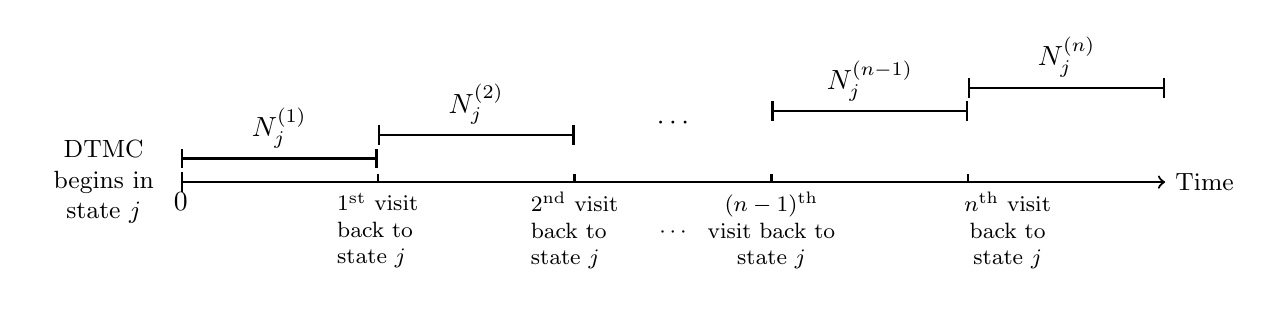
\begin{tikzpicture}[thick]
            % draw horizontal line
            \draw[|->] (0,0) -- (12.5,0);

            % draw vertical lines
            \draw (2.5, 3pt) -- (2.5, 0pt);
            \draw (5, 3pt) -- (5, 0pt);
            \draw (7.5, 3pt) -- (7.5, 0pt);
            \draw (10, 3pt) -- (10, 0pt);

            % place axis labels
            \node[anchor=north] at (0,0) {$0$};
            \node[anchor=north] at (2.5,0) {\footnotesize\begin{tabular}{l}
                    $1\textsuperscript{st}$ visit \\ back to \\ state $j$
                \end{tabular}};
            \node[anchor=north] at (5,0) {\footnotesize\begin{tabular}{l}
                    $2\textsuperscript{nd}$ visit \\ back to \\ state $j$
                \end{tabular}};
            \node[anchor=north] at (6.25,0) {\footnotesize\begin{tabular}{c}
                    \\ $\cdots$ \\
                \end{tabular}};
            \node[anchor=north] at (7.5,0) {\footnotesize\begin{tabular}{c}
                    $(n-1)\textsuperscript{th}$ \\ visit back to \\ state $j$
                \end{tabular}};
            \node[anchor=north] at (10.5,0) {\footnotesize\begin{tabular}{c}
                    $n\textsuperscript{th}$ visit \\ back to \\ state $j$
                \end{tabular}};
            \node[anchor=west] at (12.5,0) {\small Time};
            \node[anchor=east] at (0,0) {\small\begin{tabular}{c}
                    DTMC \\ begins in\\ state $j$
                \end{tabular}};

            \draw[|-|] (0,0.3) -- (2.5,0.3) node[anchor=south,midway] {$N_j^{(1)}$};
            \draw[|-|] (2.5,0.6) -- (5,0.6) node[anchor=south,midway] {$N_j^{(2)}$};
            \node at (6.25,0.75) {$\cdots$};
            \draw[|-|] (7.5,0.9) -- (10,0.9) node[anchor=south,midway] {$N_j^{(n-1)}$};
            \draw[|-|] (10,1.2) -- (12.5,1.2) node[anchor=south,midway] {$N_j^{(n)}$};
        \end{tikzpicture}
    \end{center}
\end{Regular}
